{\usebackgroundtemplate{
    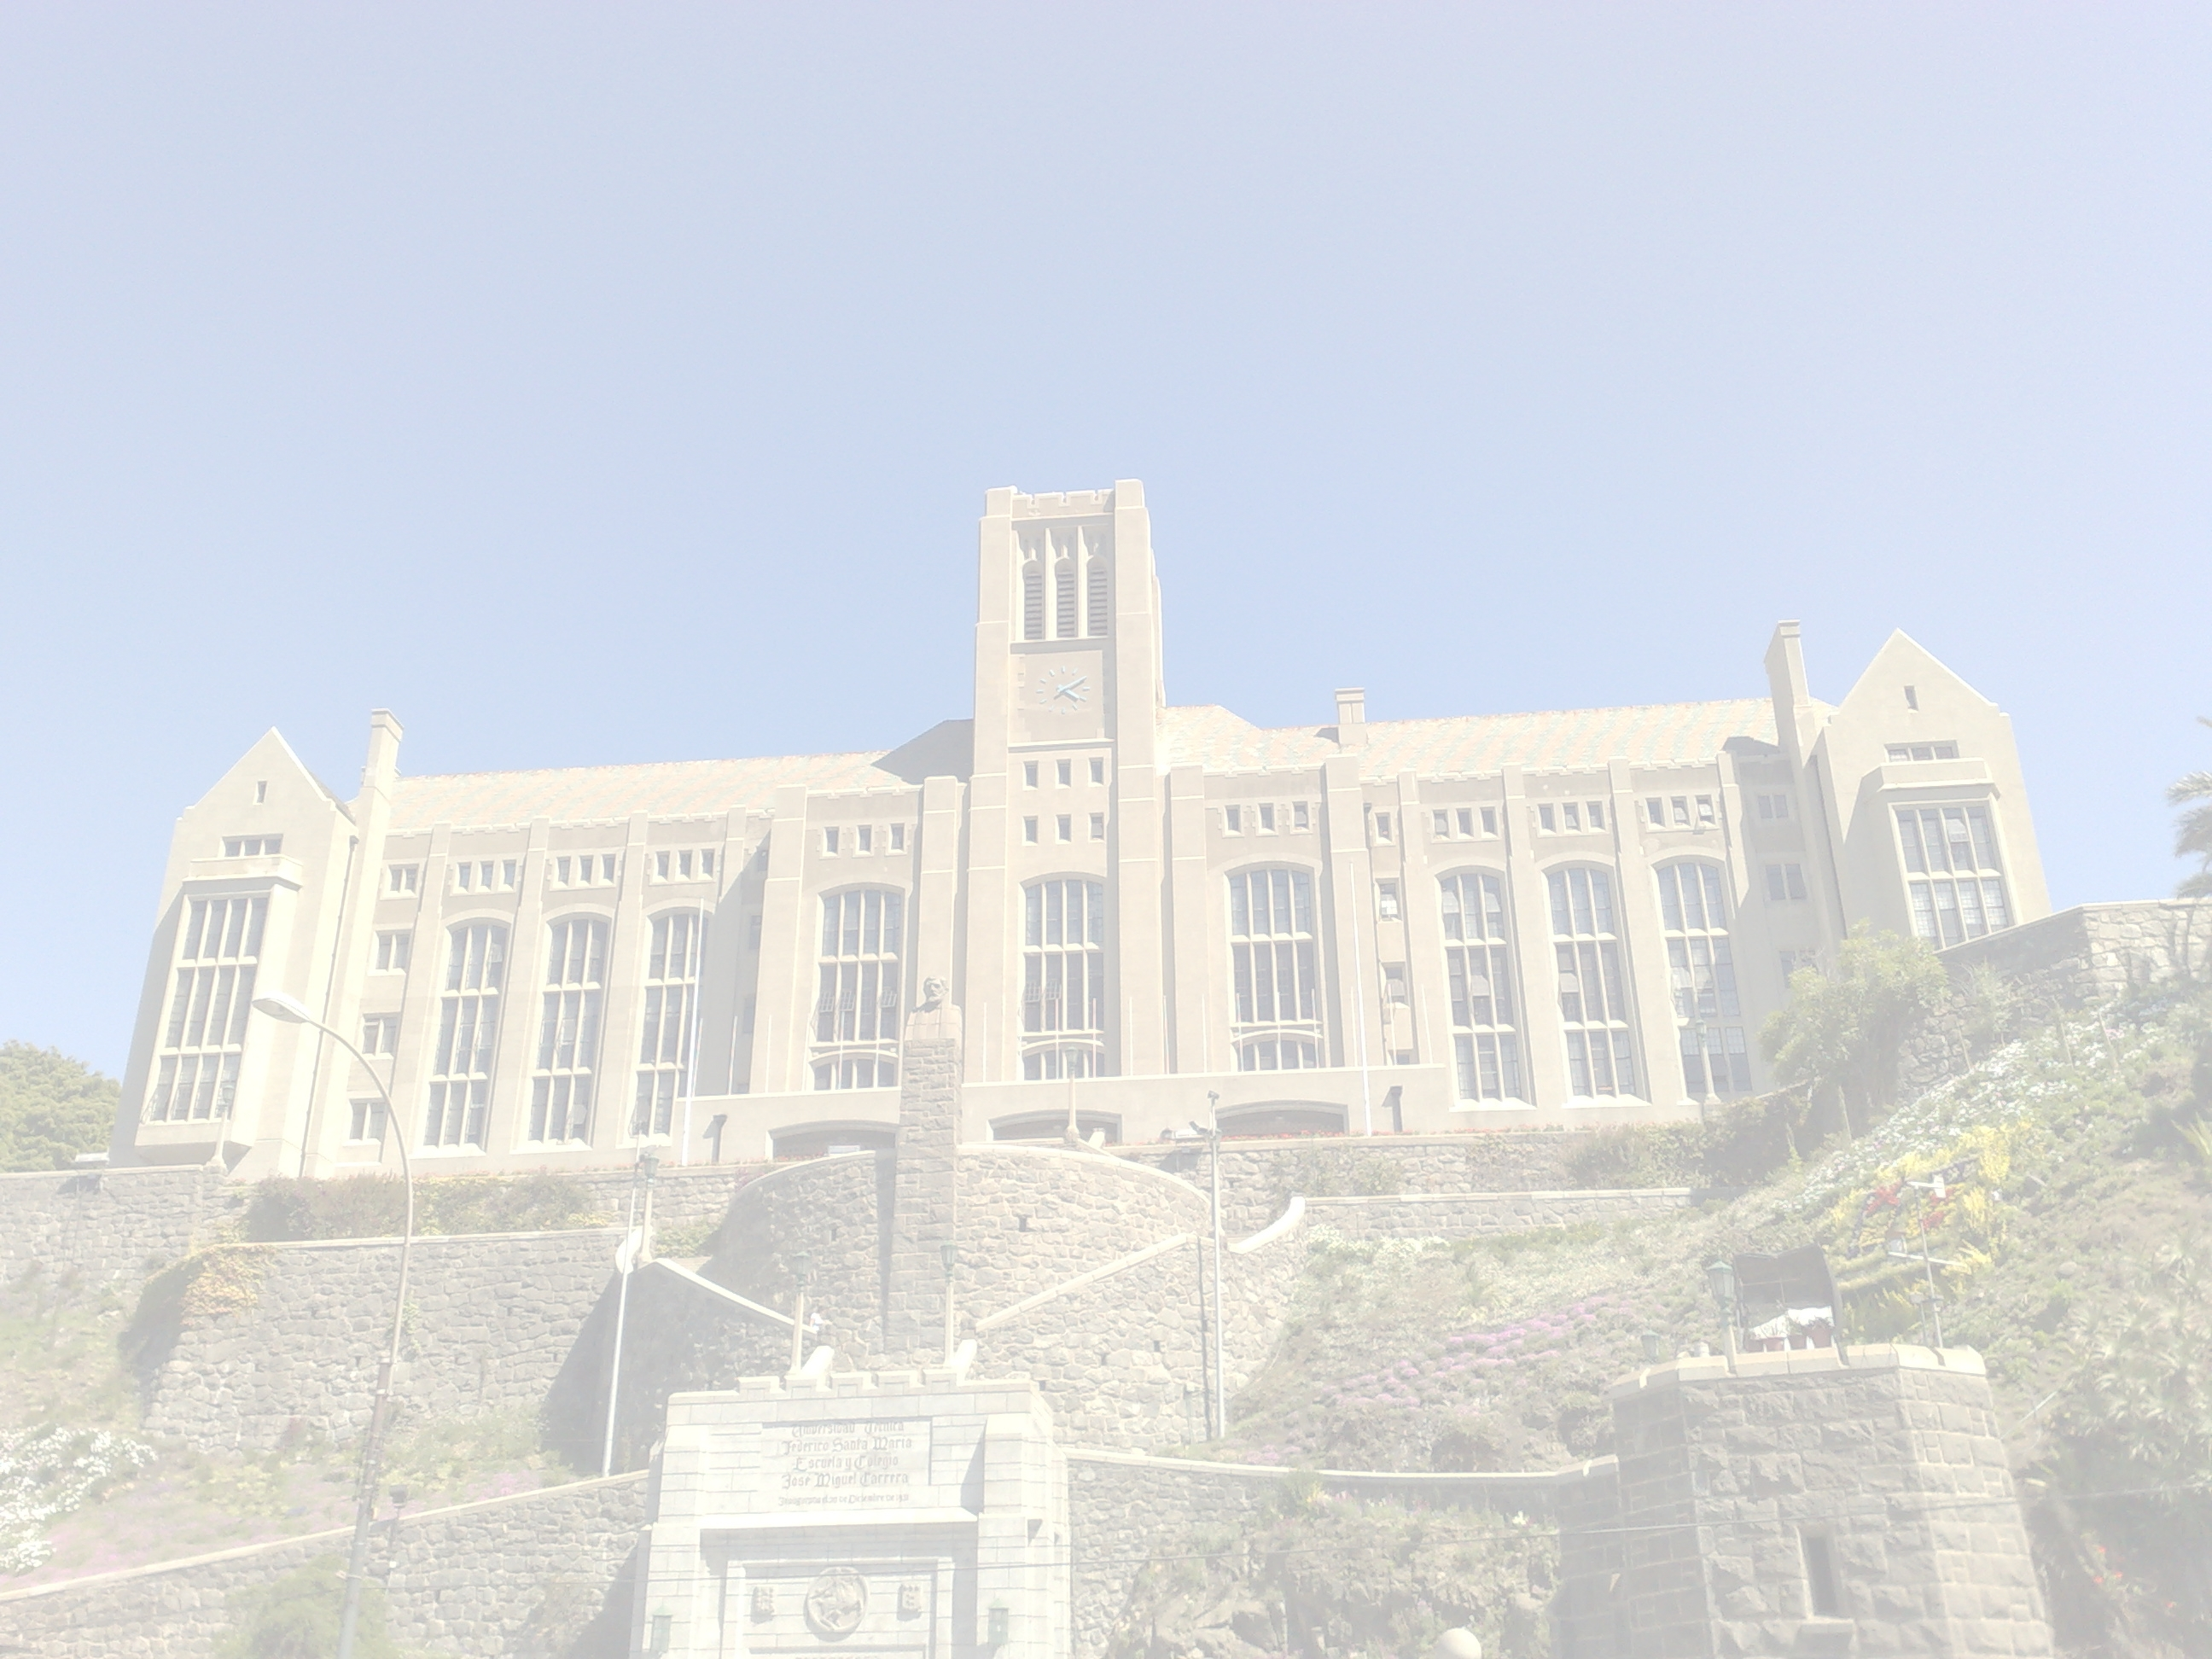
\includegraphics[width=\paperwidth,
      height=\paperheight]{Pict/UTFSM-30.jpg}
  }
  \begin{frame}
    \titlepage
  \end{frame}
}

\begin{frame}
  \frametitle{Lagrangian Formalism: Mechanics}
  Let $\{q^i\}$ be a set  functions of a parameter $t$, and $S$ be a functional of $\{q^i\}$ and their derivatives $\{\dot{q}^i\}$, defined by
  \begin{align*}
    S = \int_{t_1}^{t_f} \Lag[q,\dot{q},t].
  \end{align*}
  Assuming fixed end-points of the parameter, the condition of extreme condition for $S$ yields
  \begin{align*}
    \frac{d}{dt}\(\frac{\partial\Lag}{\partial \dot{q}^i}\)-\frac{\partial\Lag}{\partial {q}^i}=0,
  \end{align*}
  known as the Euler-Lagrange equations.
  
\end{frame}


\begin{frame}
  \frametitle{Geodesics}

  \begin{definition}
    A \alert{geodesic} is the shortest line joining to points of the space.
  \end{definition}

  \begin{columns}
    \column{.55\textwidth}
    In metric spaces,
    \begin{align*}
      ds^2(g) = g_{ab}(x) dx^a\otimes dx^b.
    \end{align*}
    Therefore, by minimising the functional 
    \begin{align*}
      S&=\int ds\\
      &= \sqrt{g_{ab}(x) dx^a\otimes dx^b},
    \end{align*}
    the geodesic equation is obtained.
    \column{.4\textwidth}
    \begin{alertblock}{Shortest$\neq$Straightest}
      In non-Euclidean spaces, the shortest line is not necessarily the straightest one, i.e., a straight line is not necessarily a geodesic.
    \end{alertblock}
  \end{columns}
\end{frame}

{\usebackgroundtemplate{
    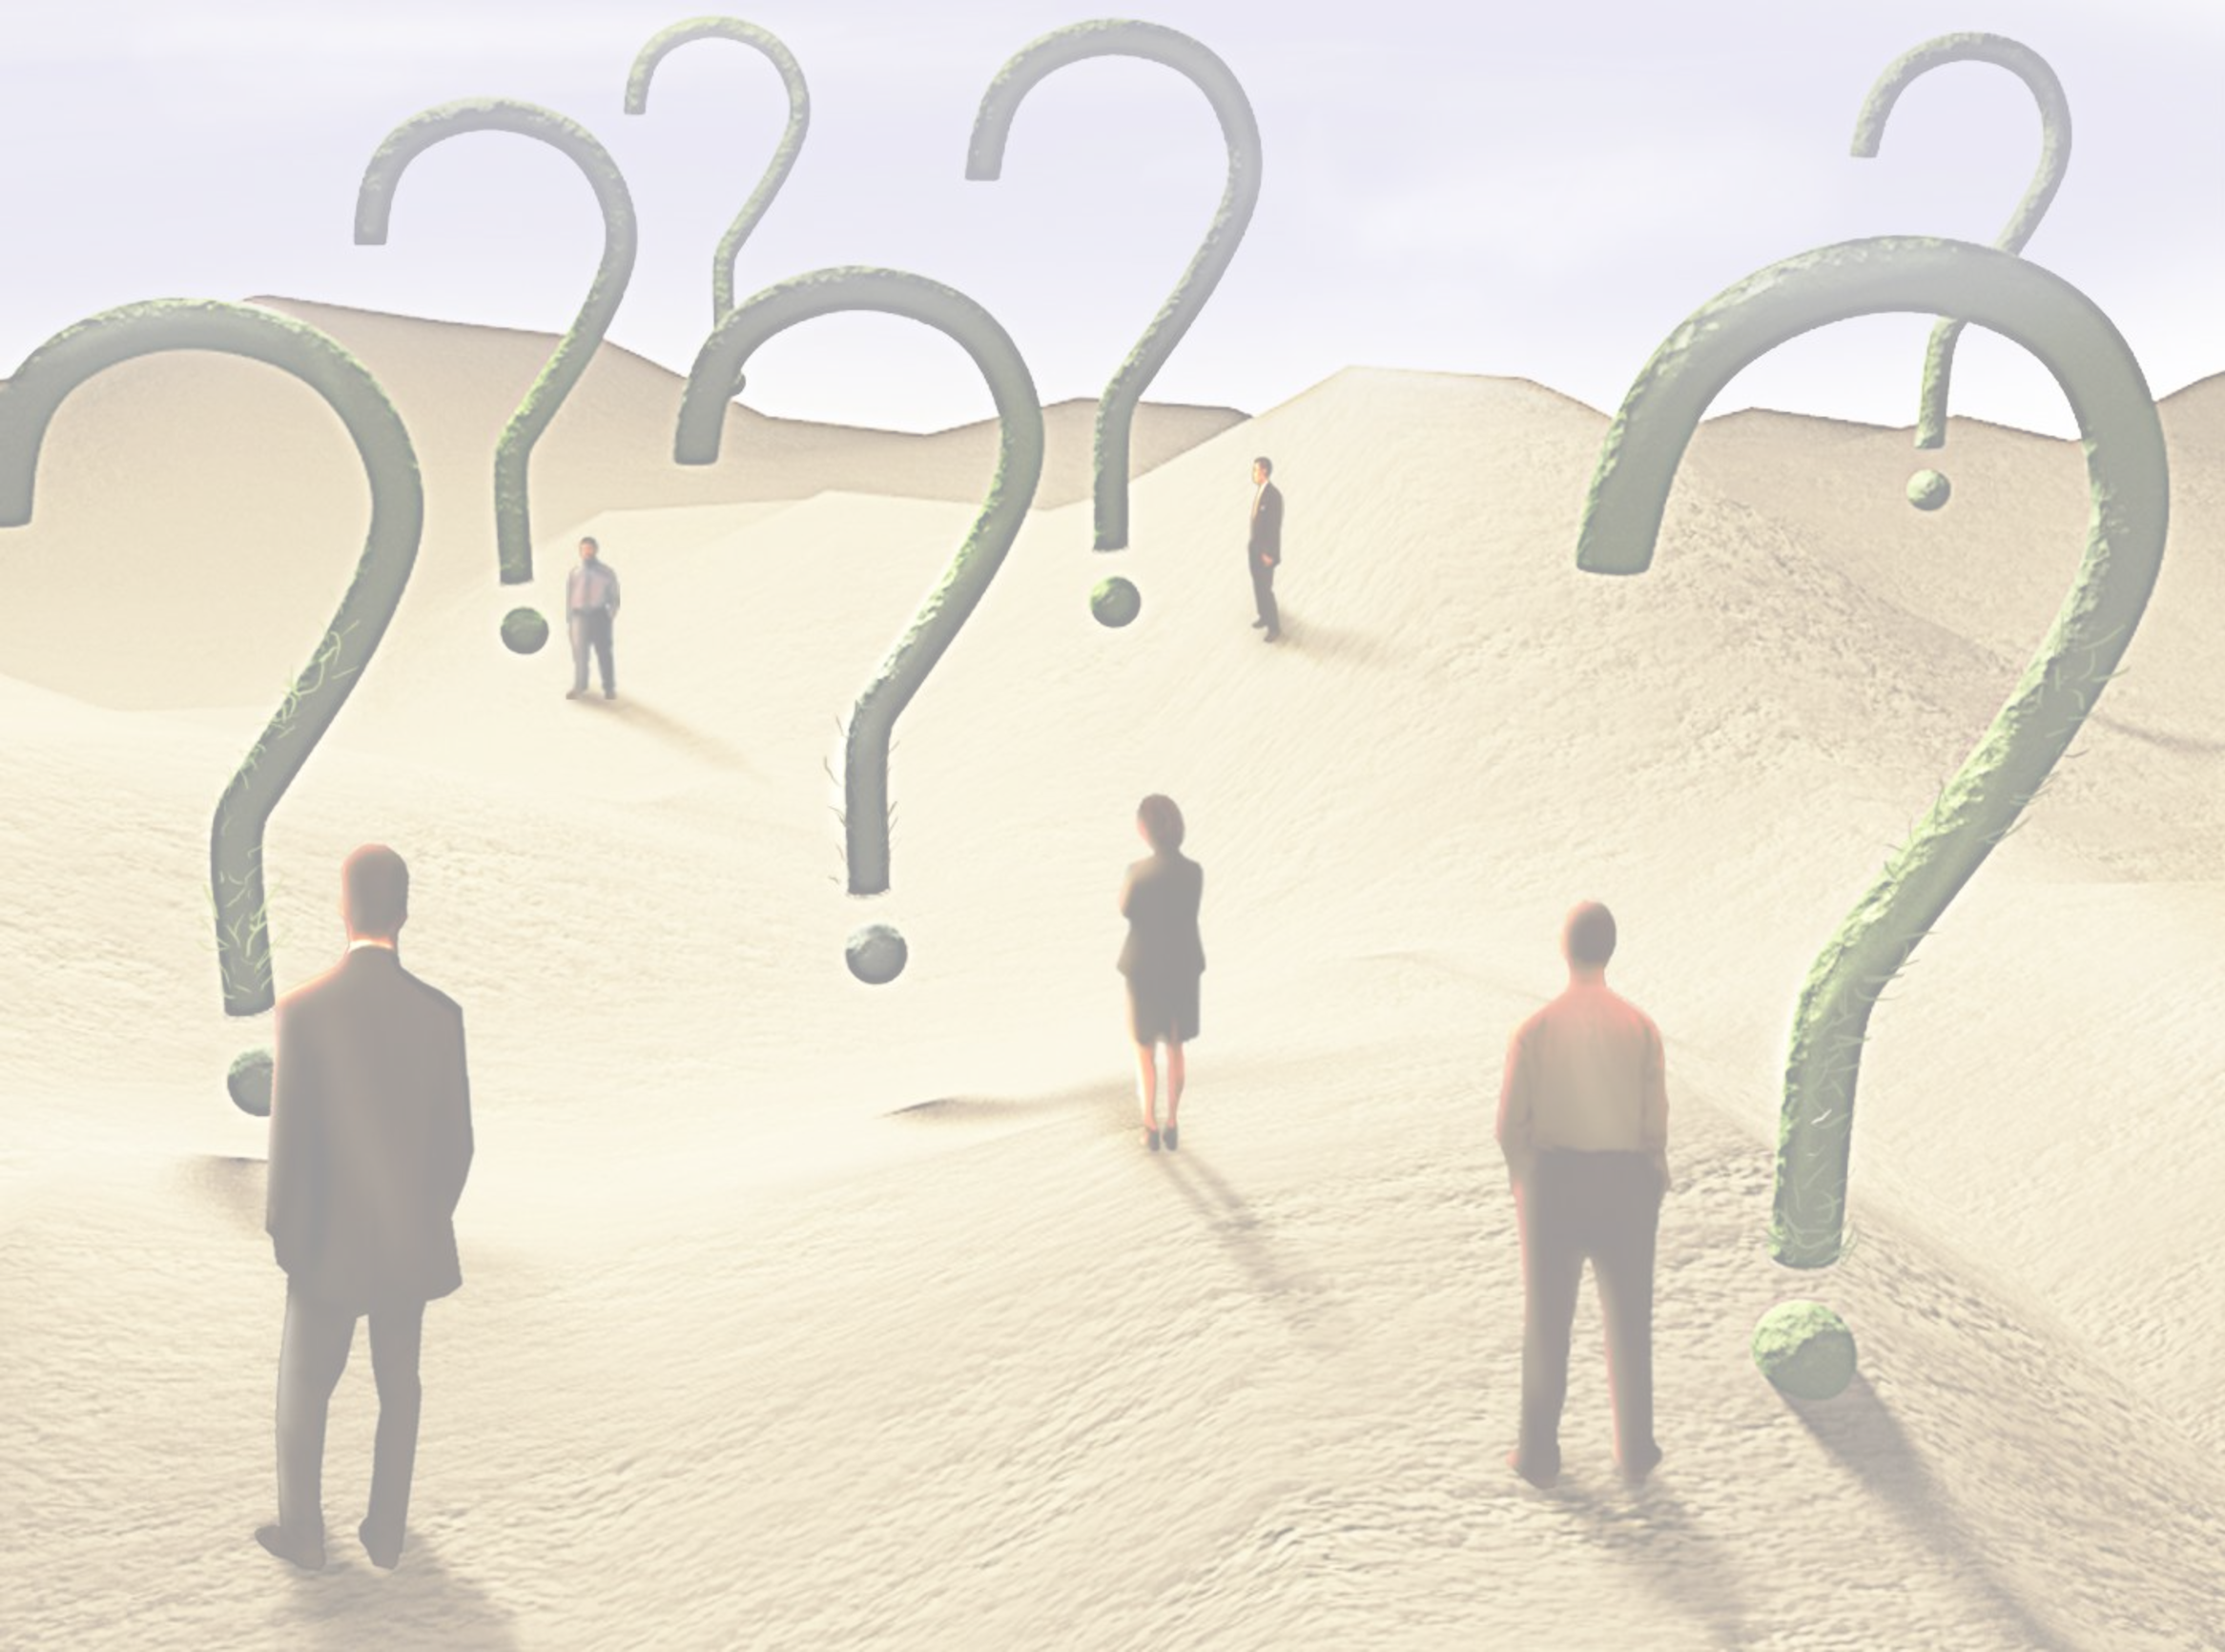
\includegraphics[width=\paperwidth,
      height=\paperheight]{Pict/Q2.pdf}
  }
  \begin{frame}
    \frametitle{\alert{WORKED EXAMPLE}}
    Find the geodesic equation.
  \end{frame}
}

